\newpage
\thispagestyle{empty}
\mbox{}

\chapter{Building a secure end-to-end pipeline}
\label{Deployment}
\section{Introduction}
This chapter has a walk-through on one of many ways to set up a secure pipeline. The pipeline starts with a source code, which will be explained further, and pushes the code to GitHub and further to \acrshort{aws}. Within these steps are the security measures and scans discussed previously. Some of these steps are automated using Terraform\footnote{Available at: \url{https://www.terraform.io/}}, which is an \gls{iac} tool using HashiCorp Configuration Language as the programming language \cite{hcl}. Terraform \acrshort{aws} Documentation\footnote{Available at: \url{https://registry.terraform.io/providers/hashicorp/aws/latest}} has been used to set up the different steps.
\\~\\
Figure \ref{fig: Pipeline in AWS} illustrates the pipeline in \acrshort{aws}, showing its structure and connection. The model is built as the different steps in the \gls{pipeline} are presented.

\vspace{2mm}
\begin{figure}[H]
    \centering
    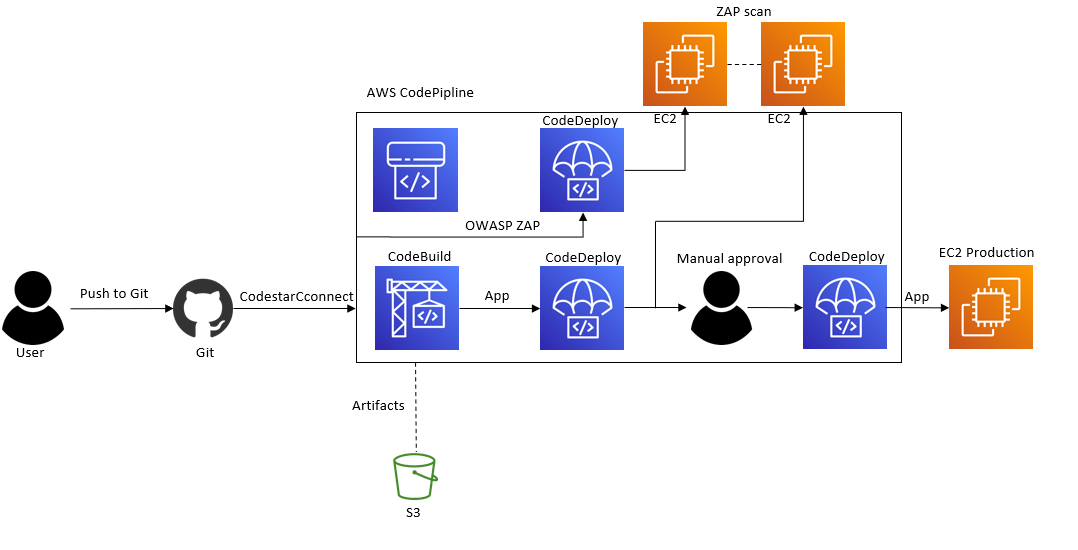
\includegraphics[width=1\columnwidth]{Images/aws-piplin-7.png}
    \caption{Pipeline in \acrshort{aws}}
    \label{fig: Pipeline in AWS}
\end{figure}

\section{Code used in the pipeline}
For testing, the group decided on using \acrshort{owasp} Juice Shop\footnote{Code available at: \url{https://github.com/juice-shop/juice-shop}}, which is a deliberately vulnerable web application that is designed to help developers and others learn about web application security concepts. The code is designed to simulate a real-world application by having common vulnerabilities within the code. The intention is to encourage users to find and exploit these vulnerabilities and increase users' understanding of web application security \cite{owaspJuiceShop}. The code in the \acrshort{owasp} Juice Shop is open source code on GitHub and is written in TypeScript, which uses a Node.js server and Angular. Angular is a TypeScript-based application framework for \gls{front-end} \cite{owaspJuiceShopCode}. The code contains different vulnerabilities, including \gls{SQL-injection}s, and \gls{Cross-site scripting}. According to its website, it has registered 101 vulnerabilities in the code.

\section{Pushing to GitHub}
Security measures must be in place when the source code is ready to be pushed to GitHub. One of the previously mentioned measurements is branch protection. Branch protection rules are easy to enable in GitHub. Enabling the rules are done for each repository. GitHub has different branch protection rules that can be enabled, which are explained in Section \ref{branchprotection}. Enabling the rules can be done in \gls{GUI} or automated using Terraform, as shown in in the GitHub repository \footnote{Code for enabling branch protection rules available at: \url{https://github.com/DCSG2900-Bachelor-thesis/Enable_Branch_Protection.git}}. 
\\~\\
Further, the commit signature has to be configured. For signing commits in GitHub, either \acrshort{ssh} or \acrshort{gpg} keys can be used. The keys need to be generated and connected to the user's GitHub account. GitHub provides documentation\footnote{Instructions on making \acrshort{gpg} or \acrshort{ssh} keys available at \url{https://docs.github.com/en/authentication/managing-commit-signature-verification/signing-commits}} on how to create \acrshort{gpg} and \acrshort{ssh} keys, as well as how to connect these keys to a GitHub account.

\vspace{2mm}
\begin{figure}[H]
  \centering
  \begin{subfigure}[H]{0.4\textwidth}
    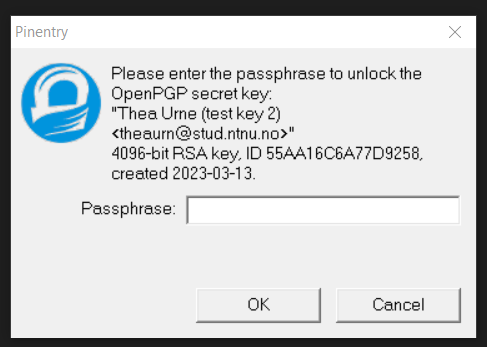
\includegraphics[width=\textwidth]{Images/signedcommits.png}
    \caption{Required passphrase when committing to GitHub}
    \label{fig:image1}
  \end{subfigure}
  \hfill
  \begin{subfigure}[H]{0.4\textwidth}
    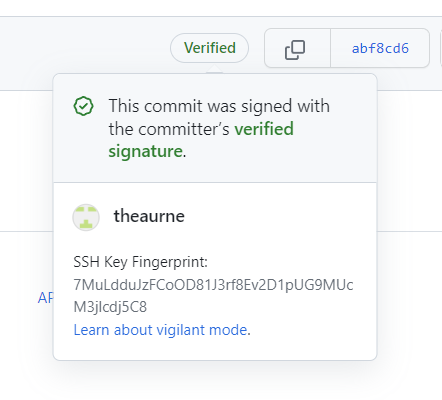
\includegraphics[width=\textwidth]{Images/verified-commit.png}
    \caption{Verified commit}
    \label{fig:image2}
  \end{subfigure}
  \caption{Required signed commits}
  \label{fig:overall}
\end{figure}

\vspace{2mm}
\begin{figure}[H]
    \centering
    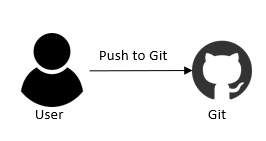
\includegraphics[width=0.5\columnwidth]{Images/aws-piplin-1.png}
    \caption{Pushing the source code to Git}
    \label{fig: Pushing the source code to Git}
\end{figure}

\section{Managing security in GitHub}
\label{Managing security in GitHub}
When the source code is securely pushed to its belonging branch and is being merged into the main branch, CodeQL needs to scan the code for vulnerabilities. This is done by setting up CodeQL\footnote{Instructions on enabling CodeQL available at \url{https://docs.github.com/en/code-security/code-scanning/automatically-scanning-your-code-for-vulnerabilities-and-errors/configuring-code-scanning-for-a-repository}} and customizing the trigger for the code scan. 
\\~\\
Setting up CodeQL is done by adding the CodeQL \acrshort{yaml} file to the workflow, which contains the configuration settings for running the analysis. Adding the pull request and push events to the workflow file customizes the trigger for the analysis, causing the analysis to run automatically whenever a pull request or push is made to the specified branch \cite{CodeQLCustom}. The branch specified in Code \ref{lst:CustomTrigger} is the main branch. 

\vspace{2mm}
\begin{lstlisting}[language=terraform, caption=Custom trigger for CodeQL alerts, captionpos=b, frame=single, label=lst:CustomTrigger]
on:
  push:
    branches: [main]
  pull_request:
    branches: [main]
\end{lstlisting}

An example on how to enable CodeQL from the \acrshort{cli} is shown in the GitHub repository FOOTNOTE.
\\~\\
Other security tools in GitHub are Dependabot\footnote{Instructions on how to enable Dependabot available at: \url{https://docs.github.com/en/code-security/dependabot/dependabot-security-updates/configuring-dependabot-security-updates}} and Secret Scanner\footnote{Instructions on how to enable Secret Scanner available at: \url{https://docs.github.com/en/code-security/secret-scanning/configuring-secret-scanning-for-your-repositories}}. These are also enabled in the security settings. Alternatively, Dependabot can be enabled from the \acrshort{cli} FOOTNOTE. After being enabled, all these tools automatically scan the code for vulnerabilities and secrets.

\vspace{2mm}
\begin{figure}[H]
    \centering
    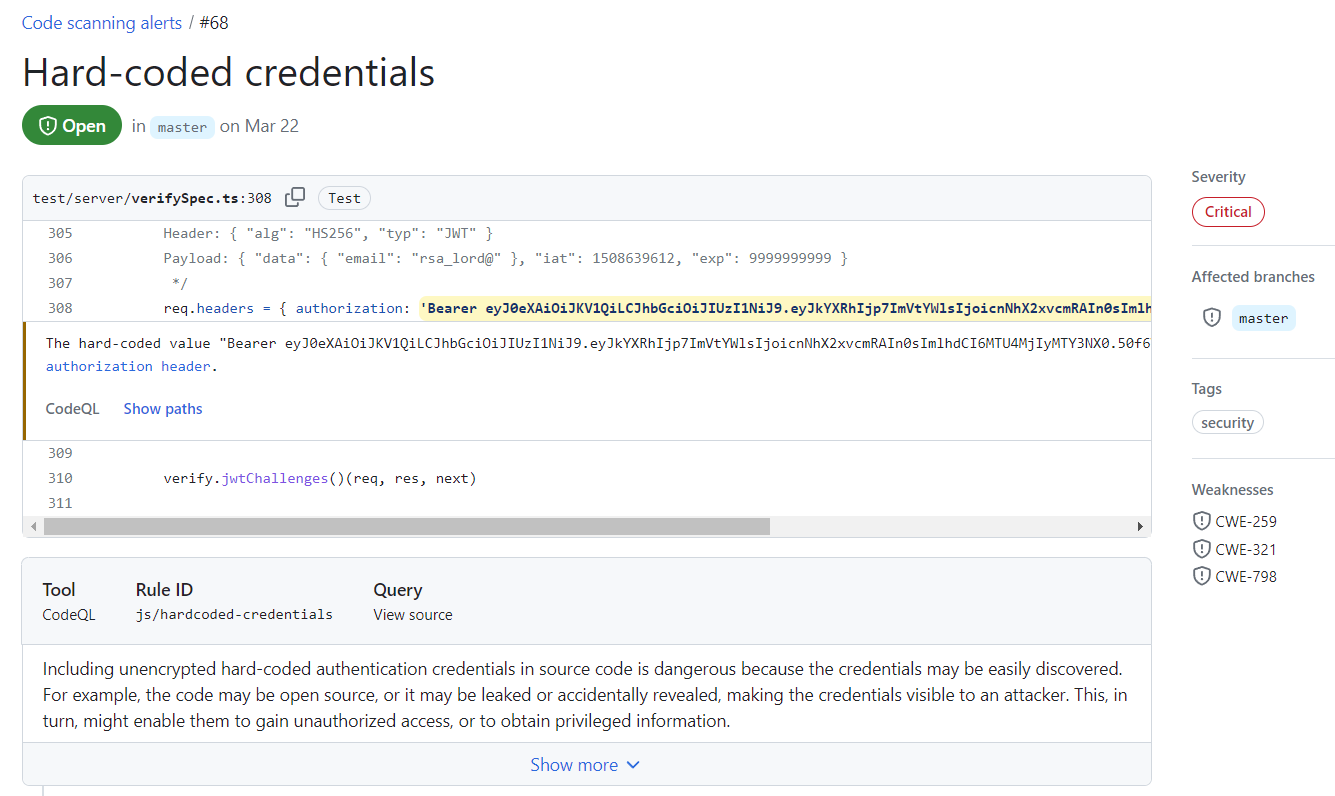
\includegraphics[width=0.8\columnwidth]{Images/codescan.png}
    \caption{Critical alert from CodeQL}
    \label{fig: Critical alert CodeQL}
\end{figure}

An example of code scanning alerts using CodeQL is the critical alert shown in Figure \ref{fig: Critical alert CodeQL}, notifying the user of a hard-coded credential. The alert is shown in a pull request from a branch to the main branch. The code scanning alerts refer to \acrshort{cwe} weaknesses, which are explained further in Section \ref{cwe}.

\vspace{2mm}
\begin{figure}[H]
    \centering
    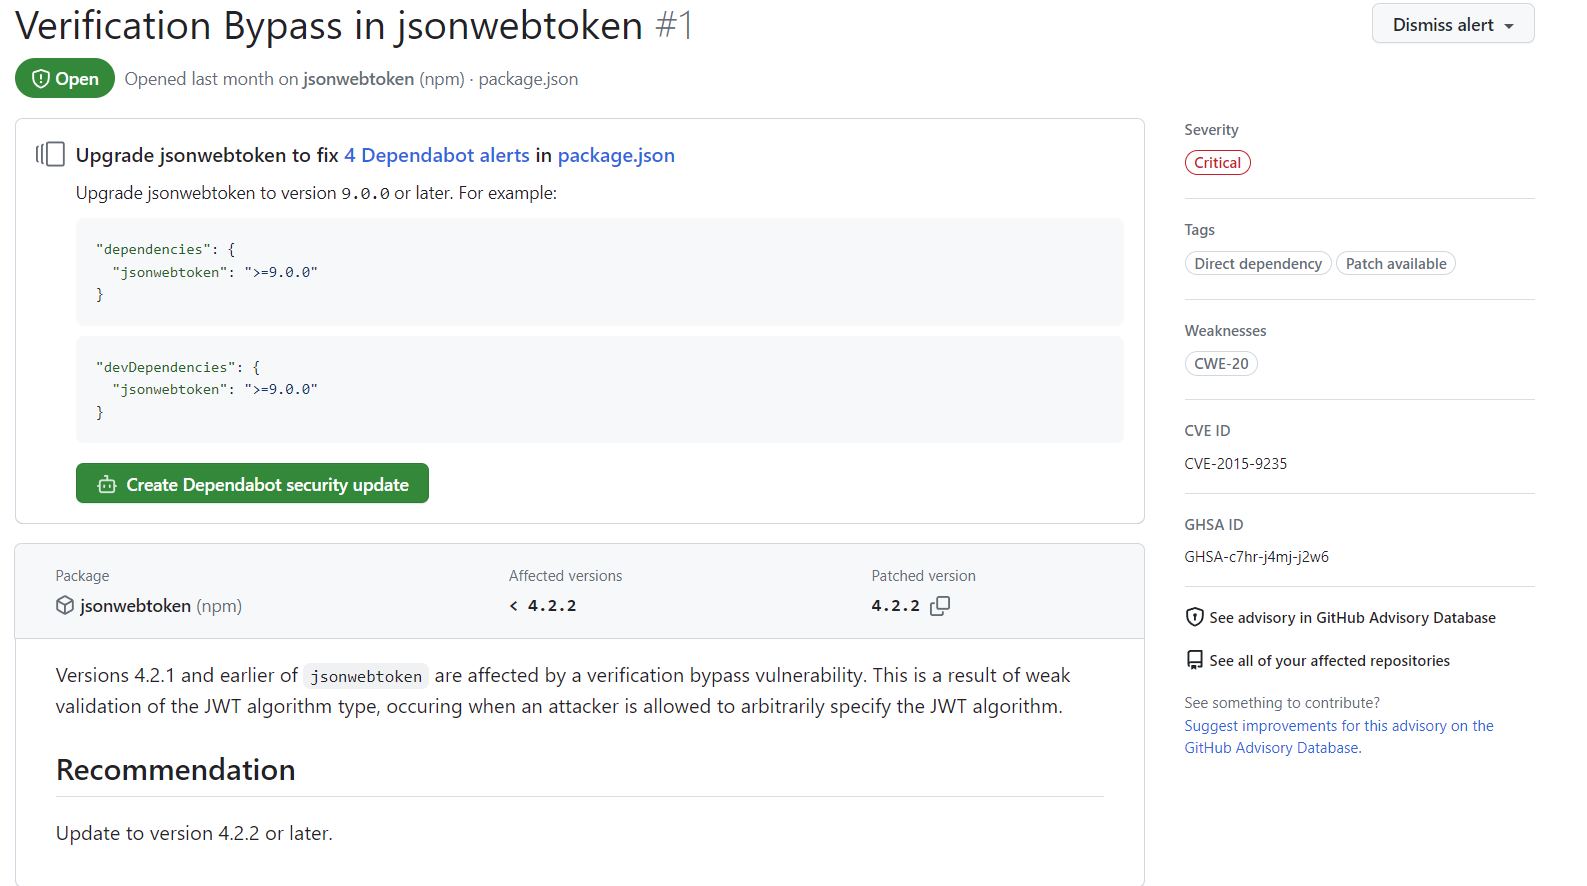
\includegraphics[width=0.8\columnwidth]{Images/dependabotalert.png}
    \caption{Critical alert from Dependabot}
    \label{fig: Critical alert from Dependabot}
\end{figure}

Figure \ref{fig: Critical alert from Dependabot} shows one of the critical alerts from Dependabot in the Juice-Shop repository. It shows a vulnerability in the dependency version used, following a suggestion on a patched version. Dependabot, similarly to CodeQL, refers to \acrshort{cwe} weaknesses. Additionally, it refers to a \acrshort{cve} ID, which is explained further in Section \ref{Common Vulnerabilities and Exposures}.

\vspace{2mm}
\begin{figure}[H]
    \centering
    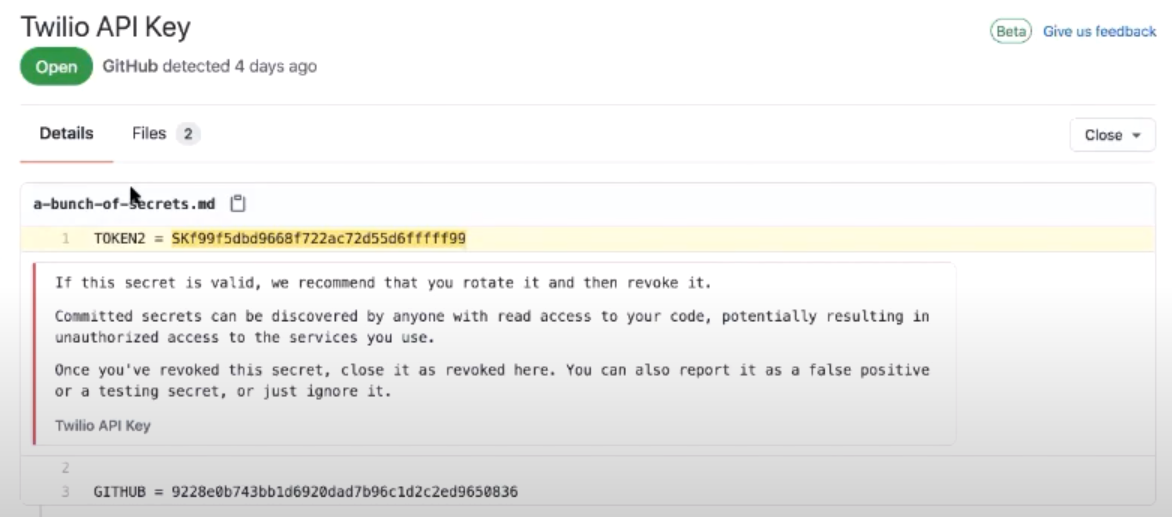
\includegraphics[width=0.8\columnwidth]{Images/secretscanneralert.png}
    \caption{Alert from secret scanner} \cite{GitHubVideo}
    \label{fig: Alert from secret scanner}
\end{figure}

The GitHub Secret Scanner did not detect any secrets in the Juice-Shop repository. Therefore, Figure \ref{fig: Alert from secret scanner} is taken from GitHub's demonstration of the secret scanner \cite{GitHubVideo}. The alert warns the user about an \acrshort{api} key that matches the pattern of their partner Twilio. 

\section{Retrieving the source code in AWS}
When the source code is pushed to the main branch in the GitHub repository, the source code can be built in \acrshort{aws}. For this to be done, a connection between the \acrshort{aws} and the GitHub account needs to be made. The connection can be made using \acrshort{aws} CodeStar Connections\footnote{A tool that enables CodePipeline to connect to third-party repositories \cite{CodeStarConnections}.}. The connection is used by \acrshort{aws} CodePipeline to automatically trigger the \gls{pipeline} in response to any changes made to the GitHub repository. A connection can be created on the \acrshort{aws} website or by using Terraform to create a connection resource with GitHub as the provider.

\vspace{2mm}
\begin{lstlisting}[language=terraform, caption=Creation of a connection between AWS and GitHub, captionpos=b, frame=single]
resource"aws_codestarconnections_connection""code-connection"{
  name          = "code-connection"
  provider_type = "GitHub" 
}
\end{lstlisting}

After successfully creating the connection resource, it is necessary to perform a manual verification process in \acrshort{aws}. This step is crucial because it is impossible to pass secrets through \acrshort{aws} to GitHub login, as the connection opens a third-party login page that \acrshort{aws} does not control.

\vspace{2mm}
\begin{figure}[H]
    \centering
    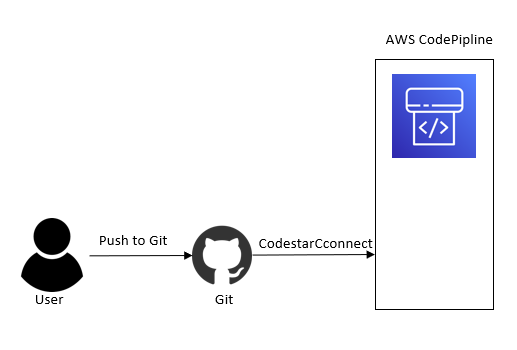
\includegraphics[width=0.6\columnwidth]{Images/aws-piplin-2-1.png}
    \caption{Committing the source code to \acrshort{aws}}
    \label{fig: Committing the source code to AWS}
\end{figure}

\section{Storing artifacts}
To store \gls{artifact}s generated during the different stages of the \gls{pipeline}, an S3 bucket is created. The bucket is created as a resource with optional variables. One crucial aspect to consider is the need for unique bucket names within the server area, as \acrshort{aws} uses this to differentiate between buckets owned by different users. The name can be configured, like in Code \ref{lst:CreateBucket}, or the name variable can be excluded, and \acrshort{aws} will configure the name themselves.

\vspace{2mm}
\begin{lstlisting}[language=terraform, caption=Creation of an S3 Bucket, captionpos=b, frame=single, label=lst:CreateBucket]
resource "aws_s3_bucket" "codepipeline_artifact" {
  bucket = "artifact-bucket-unique-name"
}
\end{lstlisting}

Granting access to the bucket is necessary for each stage in the \gls{pipeline} to retrieve the previous stage's artifacts from the S3 bucket. Therefore, access rights need to be granted separately for each stage in the pipeline. Code \ref{lst:grantaccess} grants the CodePipeline access to S3 rules, like access to the bucket itself. 

\vspace{4mm}
\begin{lstlisting}[language=terraform, caption=Permissions to CodePipeline, captionpos=b, frame=single, label=lst:grantaccess]
statement {
    sid       = ""
    actions   = [
      "s3:GetObject",
      "s3:PutObject",
      ]
    resources = [
    "${aws_s3_bucket.codepipeline_artifact.arn}/*"
    ]
    effect    = "Allow"
}
\end{lstlisting}

\vspace{2mm}
\begin{figure}[H]
    \centering
    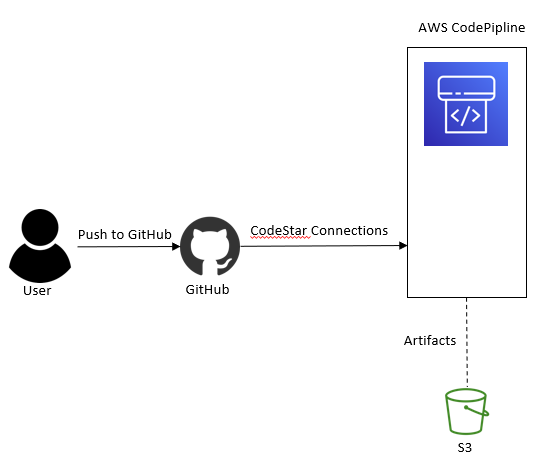
\includegraphics[width=0.6\columnwidth]{Images/aws-piplin-2.png}
    \caption{Storing the artifacts in an S3 Bucket}
    \label{fig: Storing the artifacts in an S3 Bucket}
\end{figure}

\section{Build stage}
In the build stage, CodePipeline uses CodeBuild to compile the source code into a working website \cite{CodeBuildProcess}. For the CodeBuild to run, the operating system, image, compute type and compute environment must be specified. In this example, the environment type is set to be \acrshort{aws}'s own Linux container. The compute type refers to the amount of memory, CPUs, and disk space needed, which in Code \ref{lst:CodeBuildEnvironment} is set to be the least amount of hardware resources. The combination of these variables is called a \say{build environment}.

\vspace{2mm}
\begin{lstlisting}[language=terraform, caption=Creation of a build environment, captionpos=b, frame=single, label=lst:CodeBuildEnvironment]
environment {
    compute_type                = "BUILD_GENERAL1_SMALL"
    image                       = "aws/codebuild/standard:6.0"
    type                        = "LINUX_CONTAINER"
    image_pull_credentials_type = "CODEBUILD"
}
\end{lstlisting}

Further, CodeBuild downloads the source code from the S3 bucket, which was added from the previous stage. With the source code, a \gls{buildspec} file needs to be specified to run the build.

\vspace{2mm}
\begin{figure}[H]
    \centering
    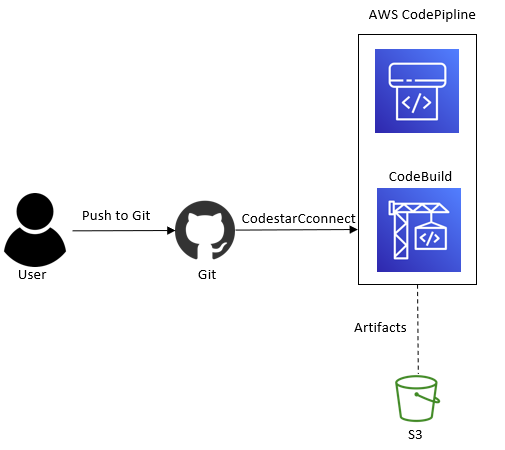
\includegraphics[width=0.6\columnwidth]{Images/aws-piplin-3.png}
    \caption{CodePipeline using CodeBuild}
    \label{fig: CodePipeline using CodeBuild}
\end{figure}

\section{Deployment to testing}
\label{Deployment to testing}
\subsection{Setting up CodeDeploy}
In order to configure CodeDeploy, the user must create an application and a deployment group. The deployment group contains settings and configurations used during the deployment. In Code \ref{lst:deployment group}, the settings specify a preset configuration. Such configuration is a set of rules and conditions, like the compute platform and conditions for failure \cite{CodeDeployConfig}. The deployment group also specifies which preconfigured instance to use for the deployment\footnote{Setting up an instance is available at \url{https://docs.aws.amazon.com/AWSEC2/latest/UserGuide/EC2_GetStarted.html}}. 

\vspace{2mm}
\begin{lstlisting}[language=terraform, caption=Creation of the deployment group, captionpos=b, frame=single, label= {lst:deployment group}]
resource "aws_codedeploy_deployment_group" "deploy_group" {
  deployment_group_name  = var.deploy_group_name
  deployment_config_name = aws_codedeploy_deployment_config.
                           deployment_config.id
  app_name               = "deployment"
  service_role_arn       = aws_iam_role.codedeploy-role.arn

  ec2_tag_filter {
    key   = "Name"
    type  = "KEY_AND_VALUE"
    value = "test_instance"
  }
}
\end{lstlisting}

As seen in Code \ref{lst:deployment group}, the deployment group specifies the application. The application is \textit{\say{a name or container used by CodeDeploy to ensure the correct revision, deployment configuration, and deployment group are referenced during a deployment}} \cite{CodeDeployApplication}. Therefore, to configure the application, it is only necessary to provide a name for it, as shown in Code \ref{lst:codedeploy application}.

\vspace{2mm}
\begin{lstlisting}[language=terraform, caption=Creation of an application for the deployment, captionpos=b, frame=single, label= lst:codedeploy application]
resource "aws_codedeploy_app" "codedeploy" {
  name = var.codedeploy_app_name
}
\end{lstlisting}

The deployment itself deploys the given revision, which typically consists of the source code for an application. In addition, an \gls{appspec} file is added to the revision. 

\subsection{Setting up for testing}

This stage utilizes two \acrshort{ec2} instances: one for \acrshort{owasp} \acrshort{zap} and the other for the application itself. Setting the scan and the application on separate instances makes it easier to manage them individually. This setup also allows for code to be reused when deploying the application into production. However, both instances utilize the same S3 bucket, but the files are separated into two different directories so they do not interfere with each other.

\vspace{2mm}
\begin{figure}[H]
    \centering
    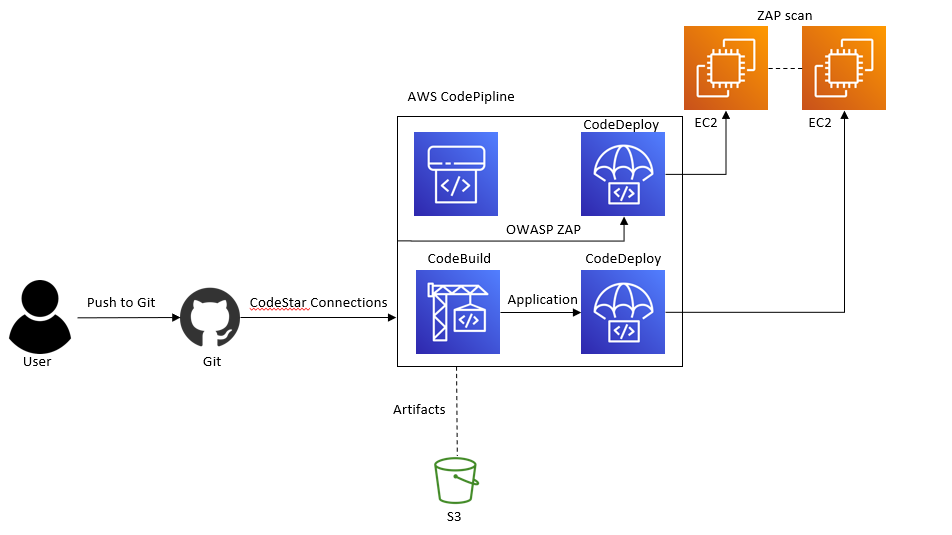
\includegraphics[width=0.6\columnwidth]{Images/aws-piplin-5.png}
    \caption{Deployment to testing}
    \label{fig: Deployment to testing}
\end{figure}

For \acrshort{owasp} \acrshort{zap} to be able to scan the application, the instances need to communicate. To enable communication between the \acrshort{ec2} instances within the \acrlong{vpc} (\acrshort{vpc}), individual network interfaces have been allocated to each instance with a single IP address. This method guarantees that both instances can find each other because the IP address will always be the same.

\vspace{2mm}
\begin{lstlisting}[language=terraform, caption=Allocation of IP adresses, captionpos=b, frame=single]
resource "aws_network_interface" "interface_network1" {
  subnet_id   = aws_subnet.my_subnet.id
  private_ips = ["172.16.10.100"]
}
resource "aws_network_interface" "interface_network2" {
  subnet_id   = aws_subnet.my_subnet.id
  private_ips = ["172.16.10.101"] 
}
\end{lstlisting}

The security tests are conducted by setting up a docker container on the \acrshort{ec2} instance created for \acrshort{owasp} \acrshort{zap}, which runs one of the automated standard tests predefined by the \acrshort{dast} tool. In addition, the container uses the \say{weekly stable image} of \acrshort{owasp} \acrshort{zap}\footnote{Available at \url{https://hub.docker.com/r/owasp/zap2docker-stable/}}. Although these tests are typically customized to suit an application's specific requirements, the predefined tests are satisfactory for this demonstration. Once the container is launched, the scan is directed towards the other instance in the \acrshort{vpc}, and the output obtained is shown in Code \ref{owasp-zap-output}.

\vspace{2mm}
\begin{lstlisting}[caption=The output of an OWASP ZAP baseline scan, captionpos=b, frame=single, label={owasp-zap-output}]
WARN-NEW: Timestamp Disclosure - Unix [10096] x 1
        http://172.16.10.100:3000/main.js (200 OK)
WARN-NEW: Cross-Domain Misconfiguration [10098] x 11
        http://172.16.10.100:3000/ (200 OK)
        http://172.16.10.100:3000/assets/public/favicon_js.ico (200 OK)
        http://172.16.10.100:3000/ftp (200 OK)
        http://172.16.10.100:3000/ftp/acquisitions.md (200 OK)
        http://172.16.10.100:3000/main.js (200 OK)
WARN-NEW: Modern Web Application [10109] x 13
        http://172.16.10.100:3000/ (200 OK)
        http://172.16.10.100:3000/home/build/routes/fileServer.js:16:13 (200 OK)
        http://172.16.10.100:3000/home/build/routes/fileServer.js:32:18 (200 OK)
        http://172.16.10.100:3000/home/build/routes/runtime.js (200 OK)
        http://172.16.10.100:3000/home/node_modules/express/lib/router/index.js:280:10 (200 OK)
WARN-NEW: Dangerous JS Functions [10110] x 2
        http://172.16.10.100:3000/main.js (200 OK)
        http://172.16.10.100:3000/vendor.js (200 OK)
FAIL-NEW: 0     FAIL-INPROG: 0  WARN-NEW: 9     WARN-INPROG: 0  INFO: 0 IGNORE: 0       PASS: 51
\end{lstlisting}


\section{Deployment to production}
In the production stage, CodePipeline utilizes CodeDeploy, as described in Section \ref{Deployment to testing}. Before the code gets moved to production, it must be accepted by manual approval by a user in \acrshort{aws}. The purpose of this step is to allow for a review of the results from the automated security tests, to ensure that no faulty code is deployed. When new code or changes have gone through testing, a notification will occur in the \acrshort{sns} topic\footnote{\acrlong{sns} (\acrshort{sns}) provides message delivery to a topic. A topic is the communication channel the users can subscribe to \cite{SNStopic}.} that is created. Someone then has to approve the code waiting to be moved to production.

\vspace{2mm}
\begin{figure}[H]
    \centering
    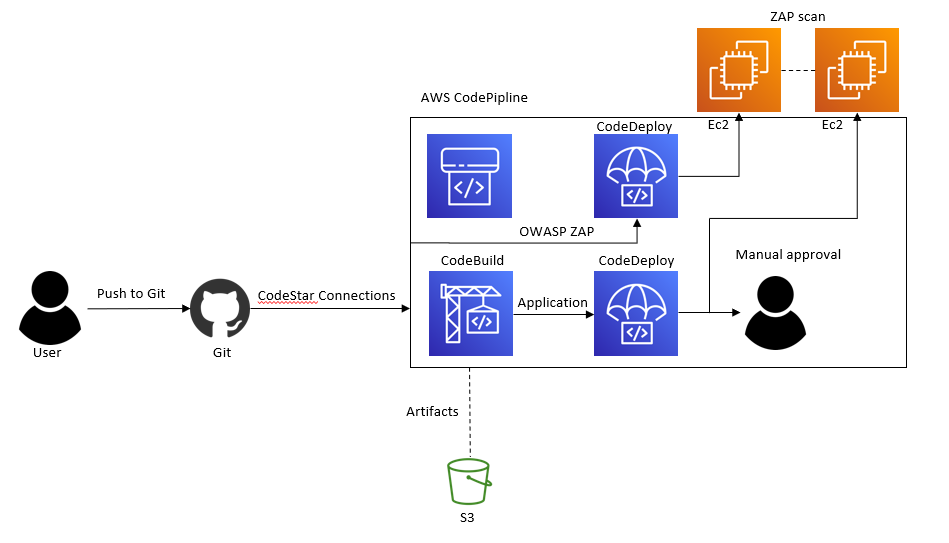
\includegraphics[width=0.8\columnwidth]{Images/aws-piplin-6.png}
    \caption{Manual approval before deploying the application}
    \label{fig: Manual approval before deploying the application}
\end{figure}

After the manual approval process is completed, the code will be deployed to production in a similar manner to the process described in Section \ref{Deployment to testing}. Figure \ref{fig: Finished pipeline created in AWS} illustrates the flow of the pipeline after completing all the necessary steps.\footnote{Complete code available at: \url{https://github.com/DCSG2900-Bachelor-thesis/CodePipeline}}

\vspace{2mm}
\begin{figure}[H]
    \centering
    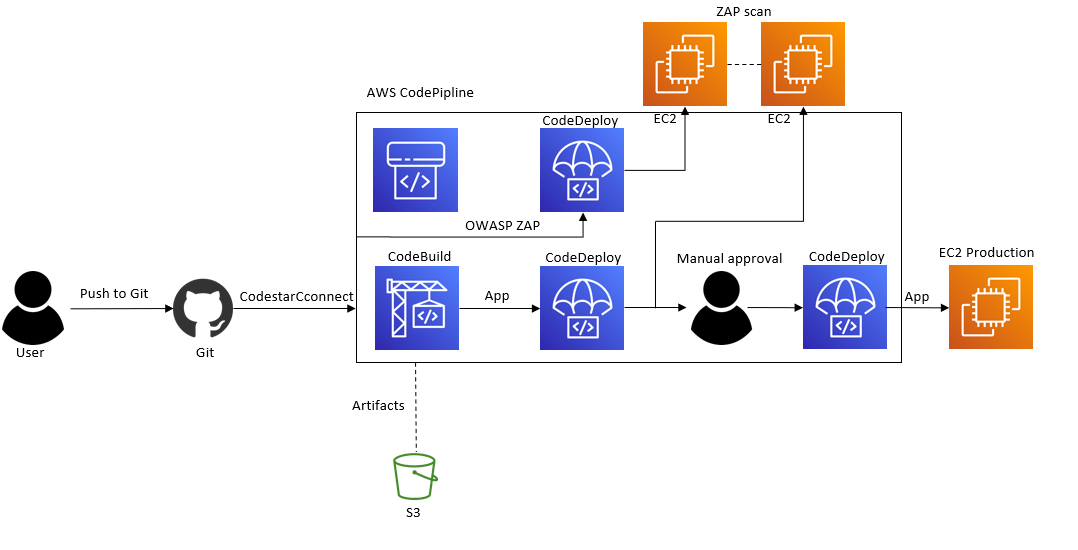
\includegraphics[width=0.8\columnwidth]{Images/aws-piplin-7.png}
    \caption{Finished pipeline created in \acrshort{aws}}
    \label{fig: Finished pipeline created in AWS}
\end{figure}